\documentclass[tikz,border=10pt]{standalone}
\usetikzlibrary{shapes}
\usetikzlibrary{arrows}
\usetikzlibrary{positioning}
\begin{document} 
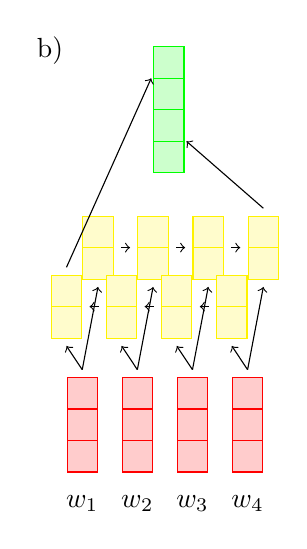
\begin{tikzpicture}[
  hid/.style 2 args={
    rectangle split,
    draw=#2,
    rectangle split parts=#1,
    fill=#2!20,
    outer sep=1mm}]

  \node[hid={4}{green}] (s2) at (2 * .7 + .4, 3) {};
  \node (s2l) at (2 *.7 +.5, 2.6) {};
  \node (s2u) at (2 *.7 +.3, 3.4) {};
  \node [anchor=west] (label) at (0, 3.75) {b)};

  \foreach \i [count=\step from 1] in {1, 2, 3, 4} {
    \node (i\step) at (.7*\step, -2) {$w_\i$};
    \node[hid={3}{red}] (e\step) at (.7*\step, -1) {};    
  }

  \foreach \step in {1,...,4} {
    \node[hid={2}{yellow}] (h_r_\step) at (-.2 + .7 *\step, .5) {};    
    \node[hid={2}{yellow}] (h_f_\step) at (.2 + .7 *\step, 1.25) {};    
    \draw[->] (e\step.north) -> (h_f_\step.south);
    \draw[->] (e\step.north) -> (h_r_\step.south);
  }
  \foreach \step/\steppp in {1/2, 2/3, 3/4} {
    \draw[->] (h_f_\step.east) -> (h_f_\steppp.west);
    \draw[->] (h_r_\steppp.west) -> (h_r_\step.east);
  }
  
  \draw[->] (h_f_4.north) -> (s2l.east);
  \draw[->] (h_r_1.north) -> (s2u.west);

\end{tikzpicture}
\end{document}
